\documentclass{presentation}

\title{yaq}
\subtitle{Instrument Shop Training}
\author{Blaise Thompson}

\institute{University of Wisconsin--Madison}
\date{\today}

\begin{document}
\maketitle

\section{Introduction}

\begin{frame}{A Typical Instrument}
  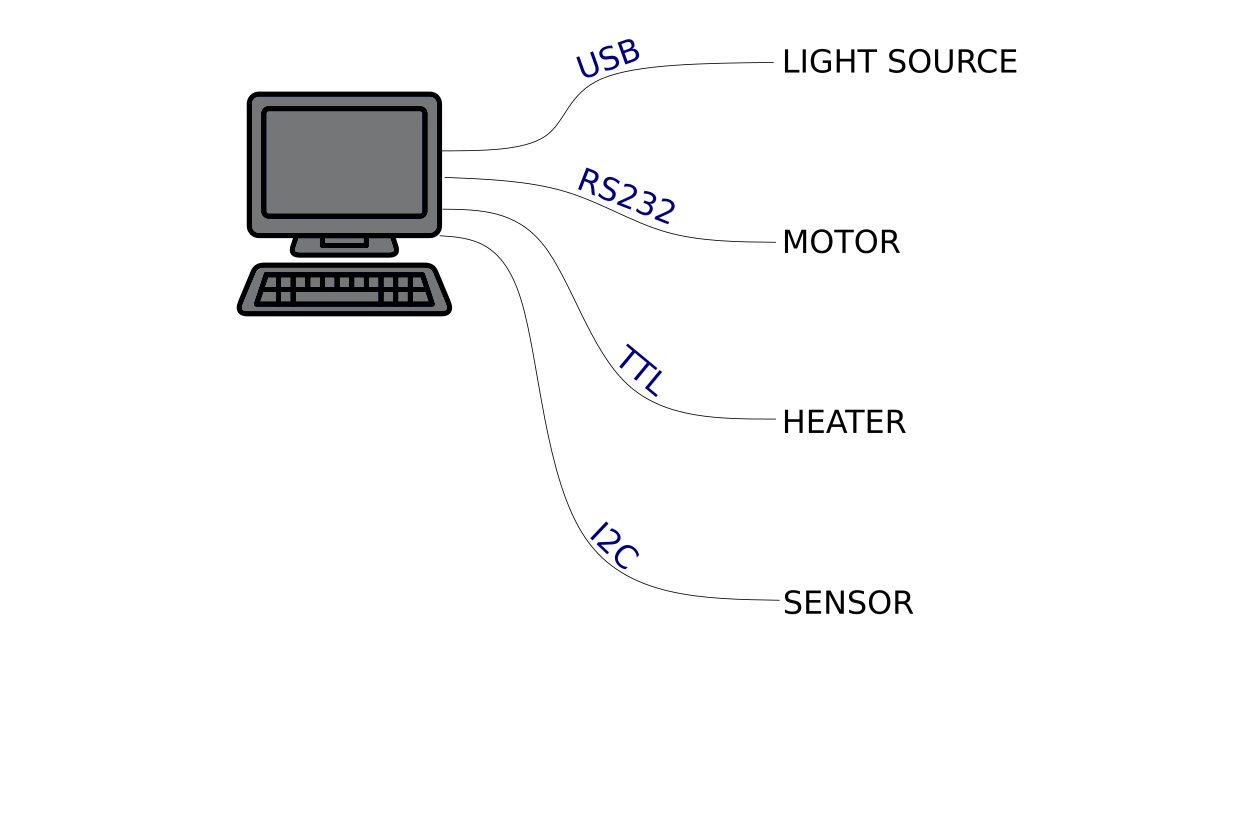
\includegraphics[width=\textwidth]{./instrument.png}
\end{frame}

\begin{frame}{A Typical Instrument}
  typical instrumental software...
  \begin{itemize}
    \item monolithic
    \begin{itemize}
      \item hard to develop---need everything to work for anything to work
      \item any one piece of the software can crash everything
      \item hard to reuse pieces in other instruments
    \end{itemize}
    \item inflexible
    \begin{itemize}
      \item lots of ``baked in'' assumptions about the particular hardware attached
      \item takes a long time to change experimental approach
    \end{itemize}
  \end{itemize}
  ... limits experimentalist freedom!
\end{frame}

\begin{frame}{The yaq Approach}
  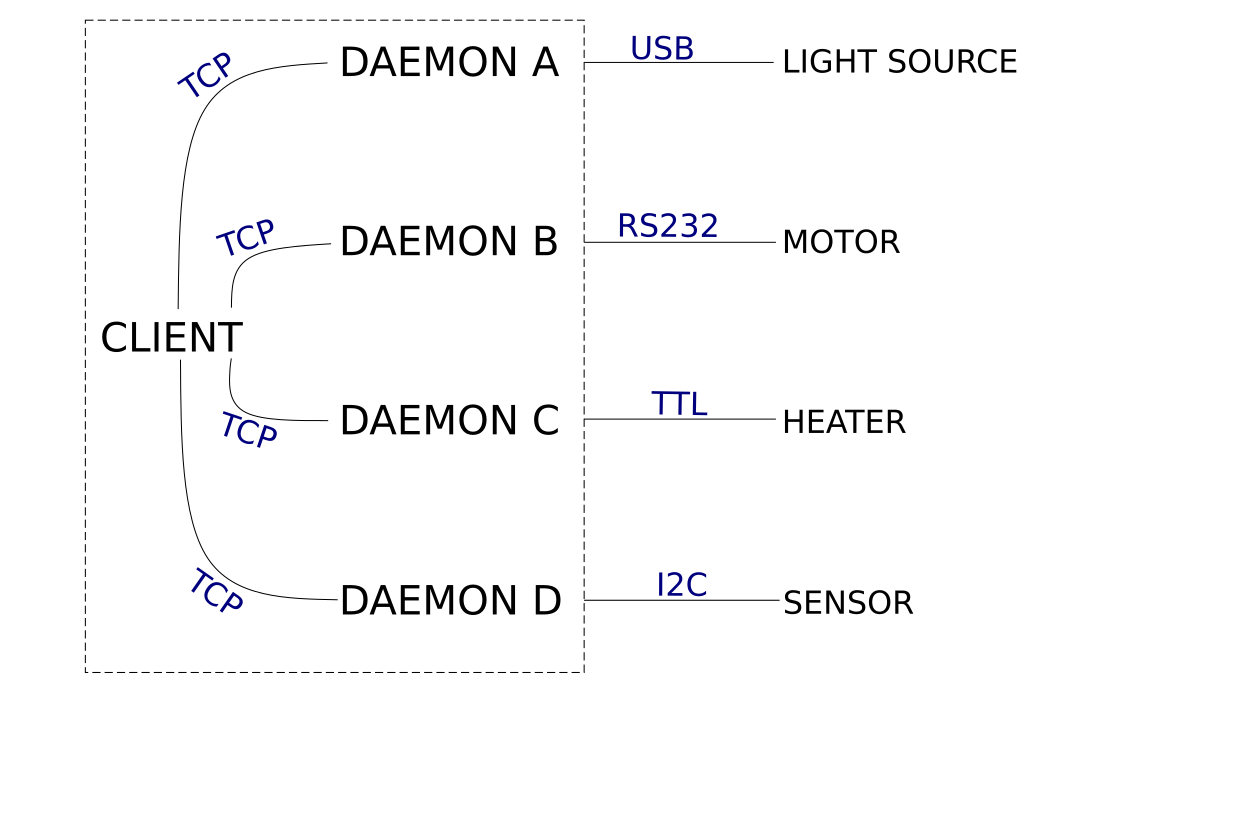
\includegraphics[width=\textwidth]{./daemons.png}
\end{frame}

\begin{frame}{The yaq Approach}
  distributed
  \begin{itemize}
    \item each daemon can be developed separately from everything else
    \item no piece of software can crash everything
    \item possibility of multiclient or networked access
  \end{itemize}
  \vfill
  portable
  \begin{itemize}
    \item reusable daemons
    \item benefit from existing ecosystem rather than ``reinventing'' hardware support
    \item use just what you need
    \item multilingual (in theory)
  \end{itemize}
\end{frame}

\begin{frame}{The yaq Approach}
  \center
  \Large{
    Guiding principle: \\
    \hl{simplify client development as much as possible} \\
    \vfill
    YOU create clients
  }
\end{frame}

\begin{frame}{The yaq Approach}
  self describing
  \begin{itemize}
    \item daemon tells the client about itself in a very structured way
    \item good documentation: \url{https://yaq.fyi}
  \end{itemize}
  \vfill
  traits
  \begin{itemize}
    \item enforce consistency between similar daemons where possible
    \item optional, extensible
  \end{itemize}
\end{frame}

\begin{frame}{The yaq Approach}
  simplify timing control
  \begin{itemize}
    \item{any daemon can be asked for ``busy'' state}
    \item{architecture removes annoyance of blocking hardware interfaces}
  \end{itemize}
\end{frame}

\section{Exercise}

\begin{frame}{yaq clients}
  using your package manager, install \texttt{yaqc}
  \begin{itemize}
    \item \texttt{client = yaqc.Client(host="192.168.1.1", port=38002)}
    \item \texttt{client.get\_position}
    \item \texttt{client.set\_position}
    \item \texttt{client.busy}
  \end{itemize}
  Try comparing across all machines!
\end{frame}

\begin{frame}{yaq clients}
  using your package manager, install \texttt{yaqd-control}
  \begin{itemize}
    \item \texttt{yaqd scan -{}-host 192.168.1.1 -{}-start 38000 \\ -{}-stop 38005}
    \item \texttt{yaqd status}
  \end{itemize}
\end{frame}

\begin{frame}{yaq clients}
  using your package manager, install \texttt{yaqc-qtpy}
  \vfill
  graphical client based on traits
\end{frame}


\begin{frame}{Test Hardware}
  \begin{columns}
    \begin{column}{0.6\textwidth}
      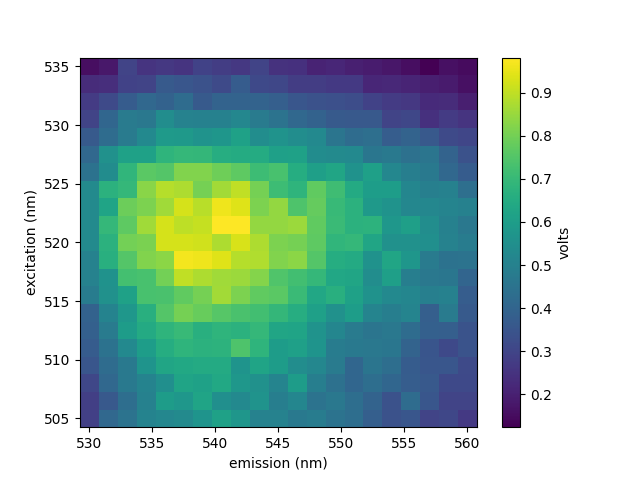
\includegraphics[width=\textwidth]{./2d-pl.png}
    \end{column}
    \begin{column}{0.4\textwidth}
      fluorescein in ethanol \\
      fluorescence
      \vfill
      using Python, take an emission slice for a given excitation wavelength
      \begin{itemize}
        \item{numpy linspace}
        \item{for loop}
        \item{matplotlib.pyplot}
      \end{itemize}
    \end{column}
  \end{columns}
\end{frame}

\section{Using yaq}

\begin{frame}{Using yaq}
  yaq doesn't have ``built in'' orchestration software
  \begin{itemize}
    \item write scripts
    \item create experiment-specific GUIs
    \item utilize existing projects focused on orchestration
  \end{itemize}
  \vfill
  the best choice depends on your instrument
  \begin{itemize}
    \item scripts are flexible and lightweight---rapid development, few users
    \item experiment-specific GUIs are great for mature experiments with many users
    \item can introduce as much or as little sophistication as needed
  \end{itemize}
  importantly you can choose a combination of many options!
\end{frame}

\begin{frame}{Bluesky}
  \center
  
\includegraphics[width=\textwidth]{./bluesky-logo.png}
  \url{https://blueskyproject.io/}
\end{frame}

\end{document}
